\documentclass{beamer}
\usepackage{caption}
\usepackage{subcaption}

\title{Conformance Checking Using Embeddings and its Applicability in the Internet of Things}
\author{Jan Kruska}
\date{\today}

\begin{document}
	\beamertemplatenavigationsymbolsempty
	\addtobeamertemplate{navigation symbols}{}{%
		\usebeamerfont{footline}%
		\usebeamercolor[fg]{footline}%
		\hspace{1em}%
		\insertframenumber
	}
	\frame{\titlepage}
	
	\begin{frame}
		\frametitle{Table of Contents}
		\tableofcontents
	\end{frame}
	\section{Motivation}
	\begin{frame}
		\frametitle{Motivation}
		\begin{itemize}
			\item We know that traditional approaches (replay and alignments) are able to measure conformance, but have some meaningful disadvantages as well.
			\item At least conceptually NLP and BPM share some important characteristics. Both deal with sequences (sentences/traces) of words/activities and aim to define similarity measures between those.
		\end{itemize}
		\begin{block}{Research Question:}
			Are adaptations of NLP techniques feasible solutions for problems in the BPM field, specifically for the problem of conformance checking.
		\end{block}
		\alert{Theoretical exploration in previous paper, here implementation and evaluation was the main concern}
	\end{frame}
	
	\section{Structure}
	\begin{frame}
		\frametitle{Structure}
		\begin{figure}
			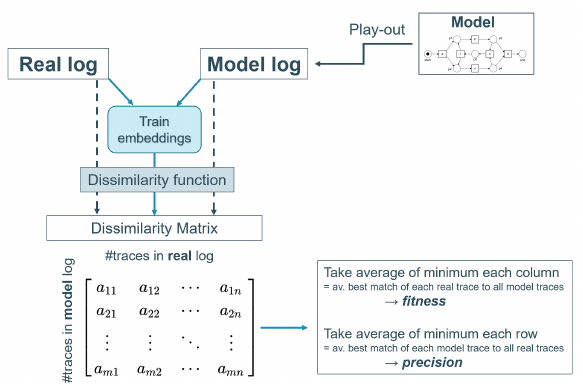
\includegraphics[width=1\textwidth]{figures/structure}
			\caption{The general structure of the approach}
			\label{fig:structure}
		\end{figure}
	\end{frame}
	
	
	\begin{frame}
		\frametitle{Used dissimilarity functions}
		\begin{enumerate}
			\item \textbf{Word Mover's distance} How much "work" is needed to transform one distribution of dirt on piles into another. Both distance between piles and amount of dirt on piles matter.
			\item \textbf{Iterative Constraint Transfers} WMD has cubic complexity in the dictionary size, which makes it unattractive. ICT is a linear time approximation of WMD obtained by relaxing one of the constraints of the LP.
			\item \textbf{\emph{trace2vec}} Analogously to \emph{doc2vec} train an embedding of bags of activities called \emph{trace2vec}. Use cosine similarity to directly compare traces in the trace embedding space.
		\end{enumerate}
	\alert{The obtained metrics are not proper fitness metrics, i.e. they do not fall within the interval $[0,1]$. As such quantitative analyses is not really possible at this point.}
	\end{frame}
	
	\section{Experiments}
	\begin{frame}
		\frametitle{Setup}
		Three experiments were performed:
		\begin{enumerate}
			\item Noise: Applying noise to a varying amount of traces/ varying amount of noise applied to same amount of traces. Investigate how the methods react. Do they deteriorate smoothly?
			\item Discovery: Discover model using different miners, determine fitness and precision using the three proposed methods as well as alignments, behavioural fitness and ETC precision.
			\item Scaling: Vary log and dictionary sizes (number of activities). Compare runtimes \alert{Sadly no runtimes of traditional methods were included.}
		\end{enumerate}
	\end{frame}
	\begin{frame}
		\frametitle{Setup}
		Random trees were generated using pm4py and the following configurations:
		
		\begin{tabular}{lll}
			Min & Mode & Max \\
			5 & 10 & 15 \\
			10 & 20 & 30 \\
			15 & 30 & 45 \\
		\end{tabular}
		\begin{tabular}{llll}
			Sequence & Parallel & Choice & Loop \\
			0.75 & 0.25 & 0 & 0 \\
			0.75 & 0 & 0.25 & 0 \\
			0.5 & 0.25 & 0.25 & 0 \\
			0.25 & 0.25 & 0.25 & 0.25 \\
		\end{tabular}
		
		Using these parameters $3\times4=12$ trees were generated.
		Then from each of those the "real" logs of 1000 traces were gathered by play-out.
		
		The scaling experiment used different unspecified trees varying the amount of activities and the size of the played-out log.
	\end{frame}
	\begin{frame}
		\frametitle{Example tree}
		\begin{figure}
			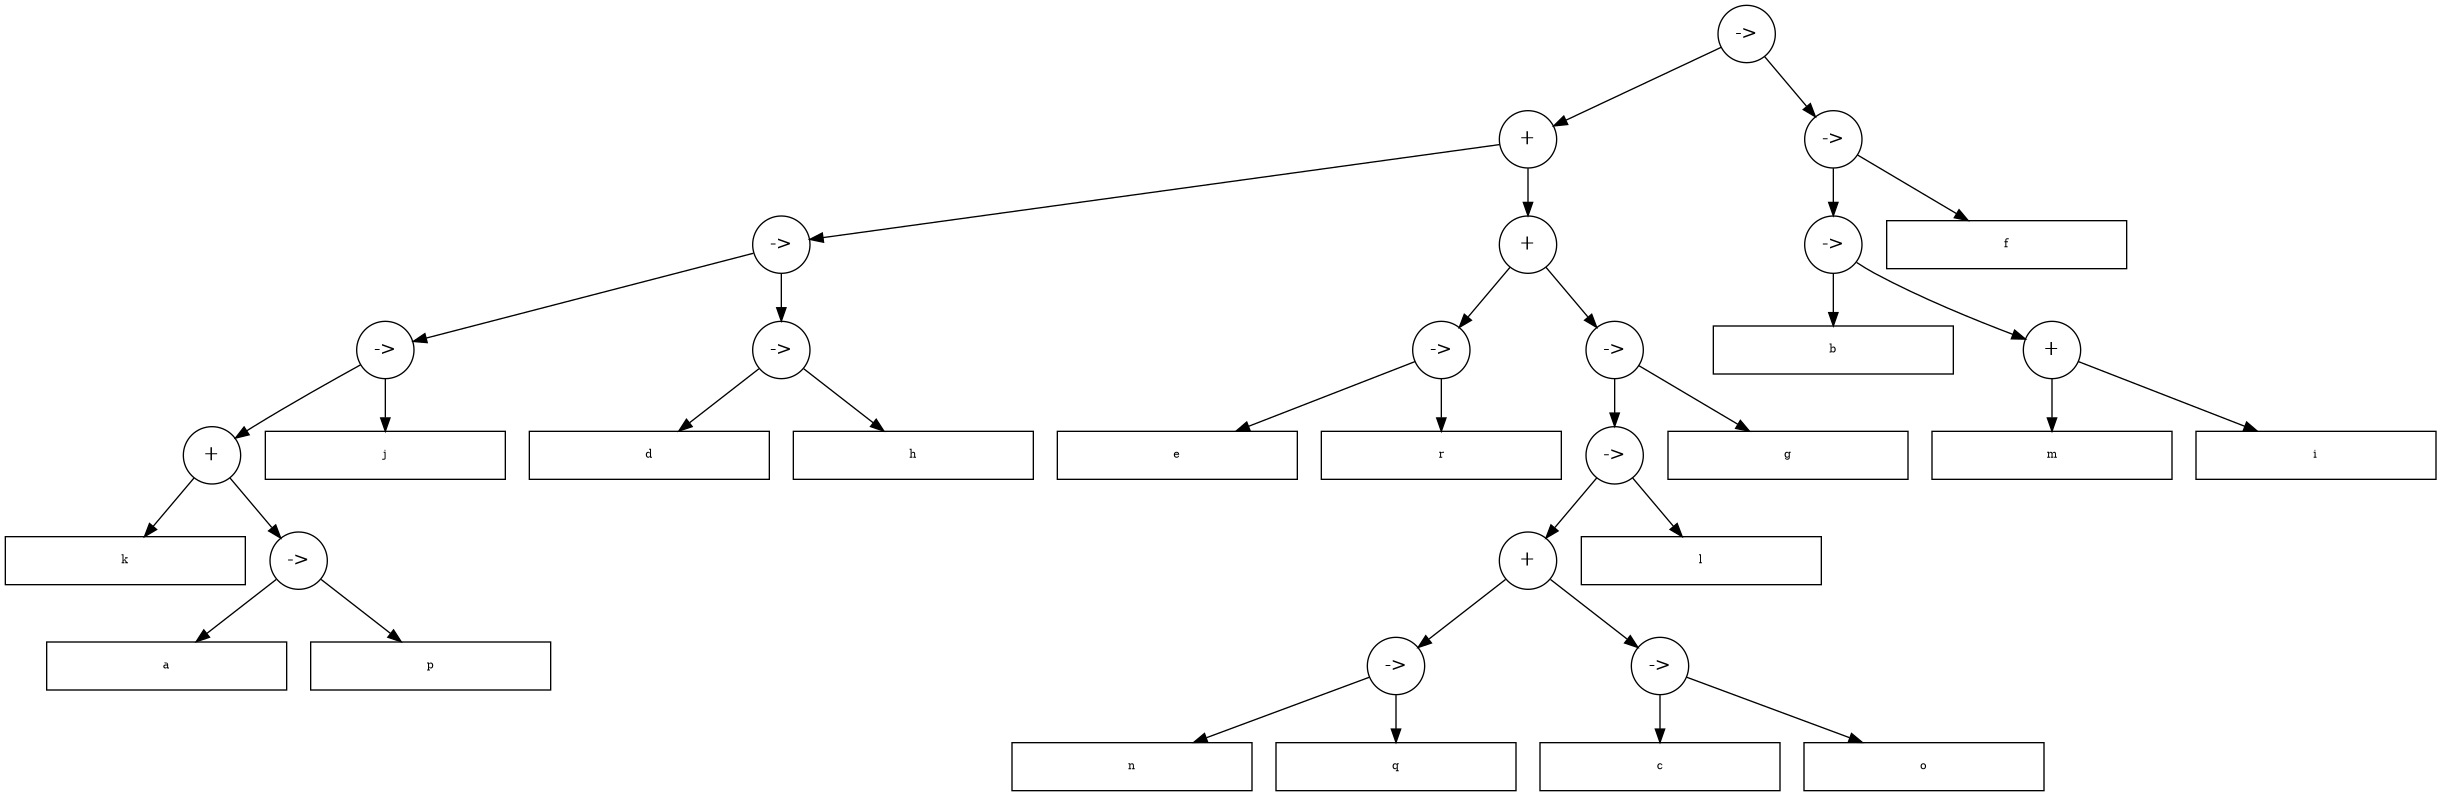
\includegraphics[width=1\textwidth]{figures/process-tree}
			\caption{A process tree generated by pm4py using parameters: Min 15, Mode 30, Max 45, sequence 0.75, parallel 0.25. }
			\label{fig:process-tree}
		\end{figure}
	\end{frame}
	
	\begin{frame}
		\frametitle{Noise}
		\begin{figure}
			\centering
			\begin{subfigure}[b]{0.49\textwidth}
				\centering
				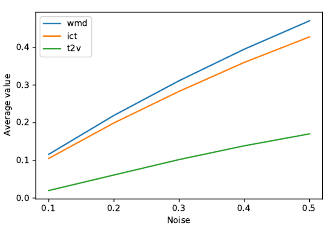
\includegraphics[width=\textwidth]{figures/noise-first}
				\caption{Average of first noise experiment (Varying trace percentage).}
				\label{fig:noise-first}
			\end{subfigure}
			\hfill
			\begin{subfigure}[b]{0.49\textwidth}
				\centering
				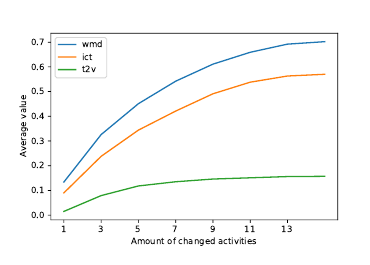
\includegraphics[width=\textwidth]{figures/noise-second}
				\caption{Average of second noise experiment (Varying amount of noise applied to trace).}
				\label{fig:noise-second}
			\end{subfigure}
		\end{figure}
	\end{frame}
	
	
	\begin{frame}
		\frametitle{Discovery}
		\begin{figure}
			\centering
			\begin{subfigure}[b]{0.49\textwidth}
				\centering
				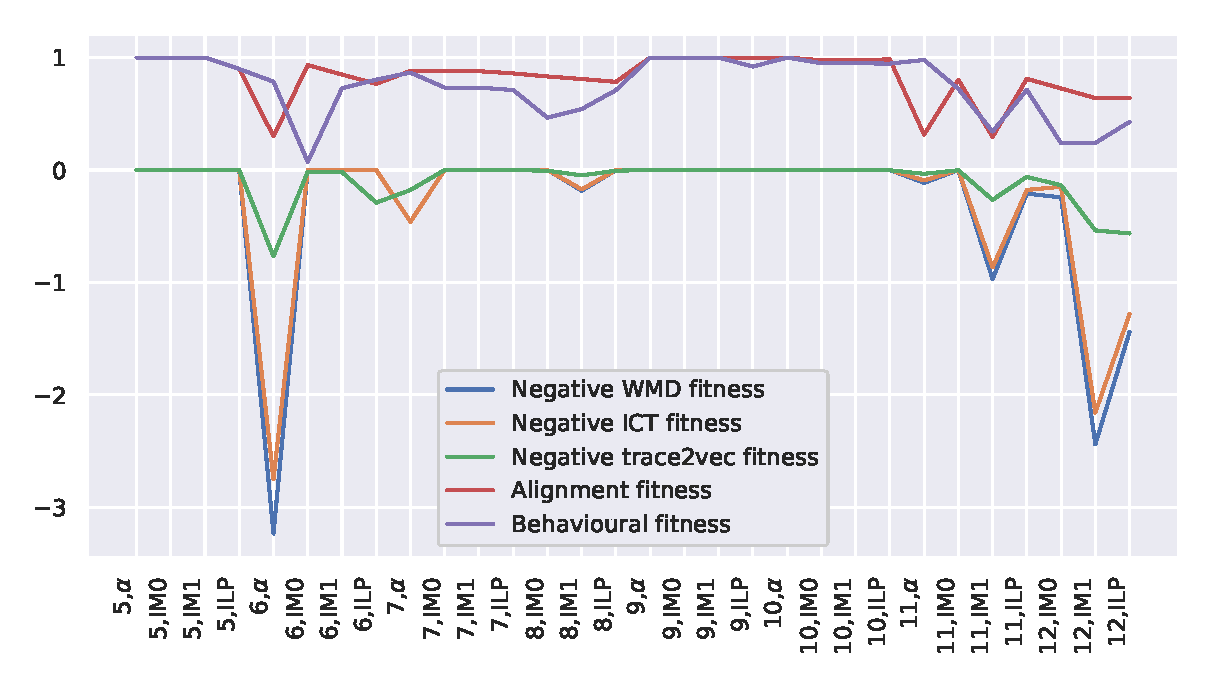
\includegraphics[width=\textwidth]{figures/fitness}
				\caption{Fitness}
				\label{fig:fitness}
			\end{subfigure}
			\hfill
			\begin{subfigure}[b]{0.49\textwidth}
				\centering
				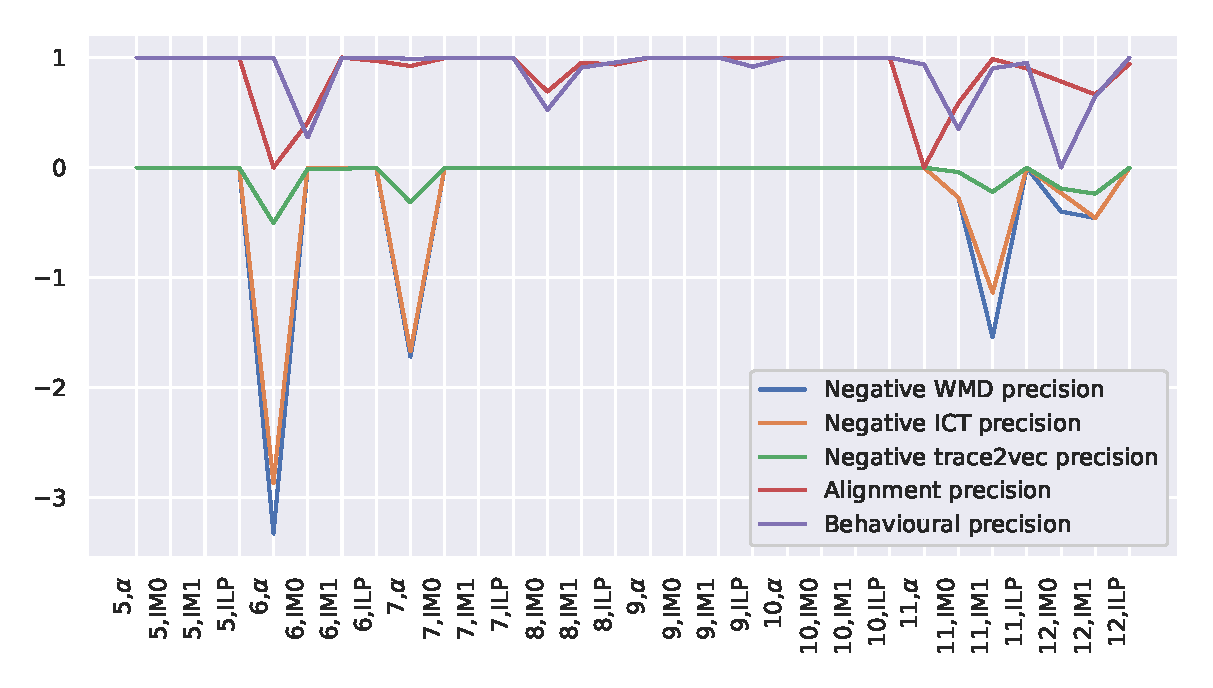
\includegraphics[width=\textwidth]{figures/precision}
				\caption{Precision}
				\label{fig:precision}
			\end{subfigure}
			\caption{Fitness and Precision for different tree, discovery technique pairings for the three proposed techniques as well as the two verification techniques.}
			\label{fig:discovery}
		\end{figure}
	\end{frame}
	
	\begin{frame}
		\frametitle{Results from Noise \& Discovery}
		\begin{itemize}
			\item Overall, noise behaves as expected
			\item Again quantitative analyses can not be made from this data!
			\item Very often the NLP and reference methods agree on perfect fitness or precision
			\item For imperfect values the methods also seem to move in a similar direction, though further research is probably needed.
		\end{itemize}
	\end{frame}
	
	
	\begin{frame}
		\frametitle{Scaling}
		\begin{figure}
			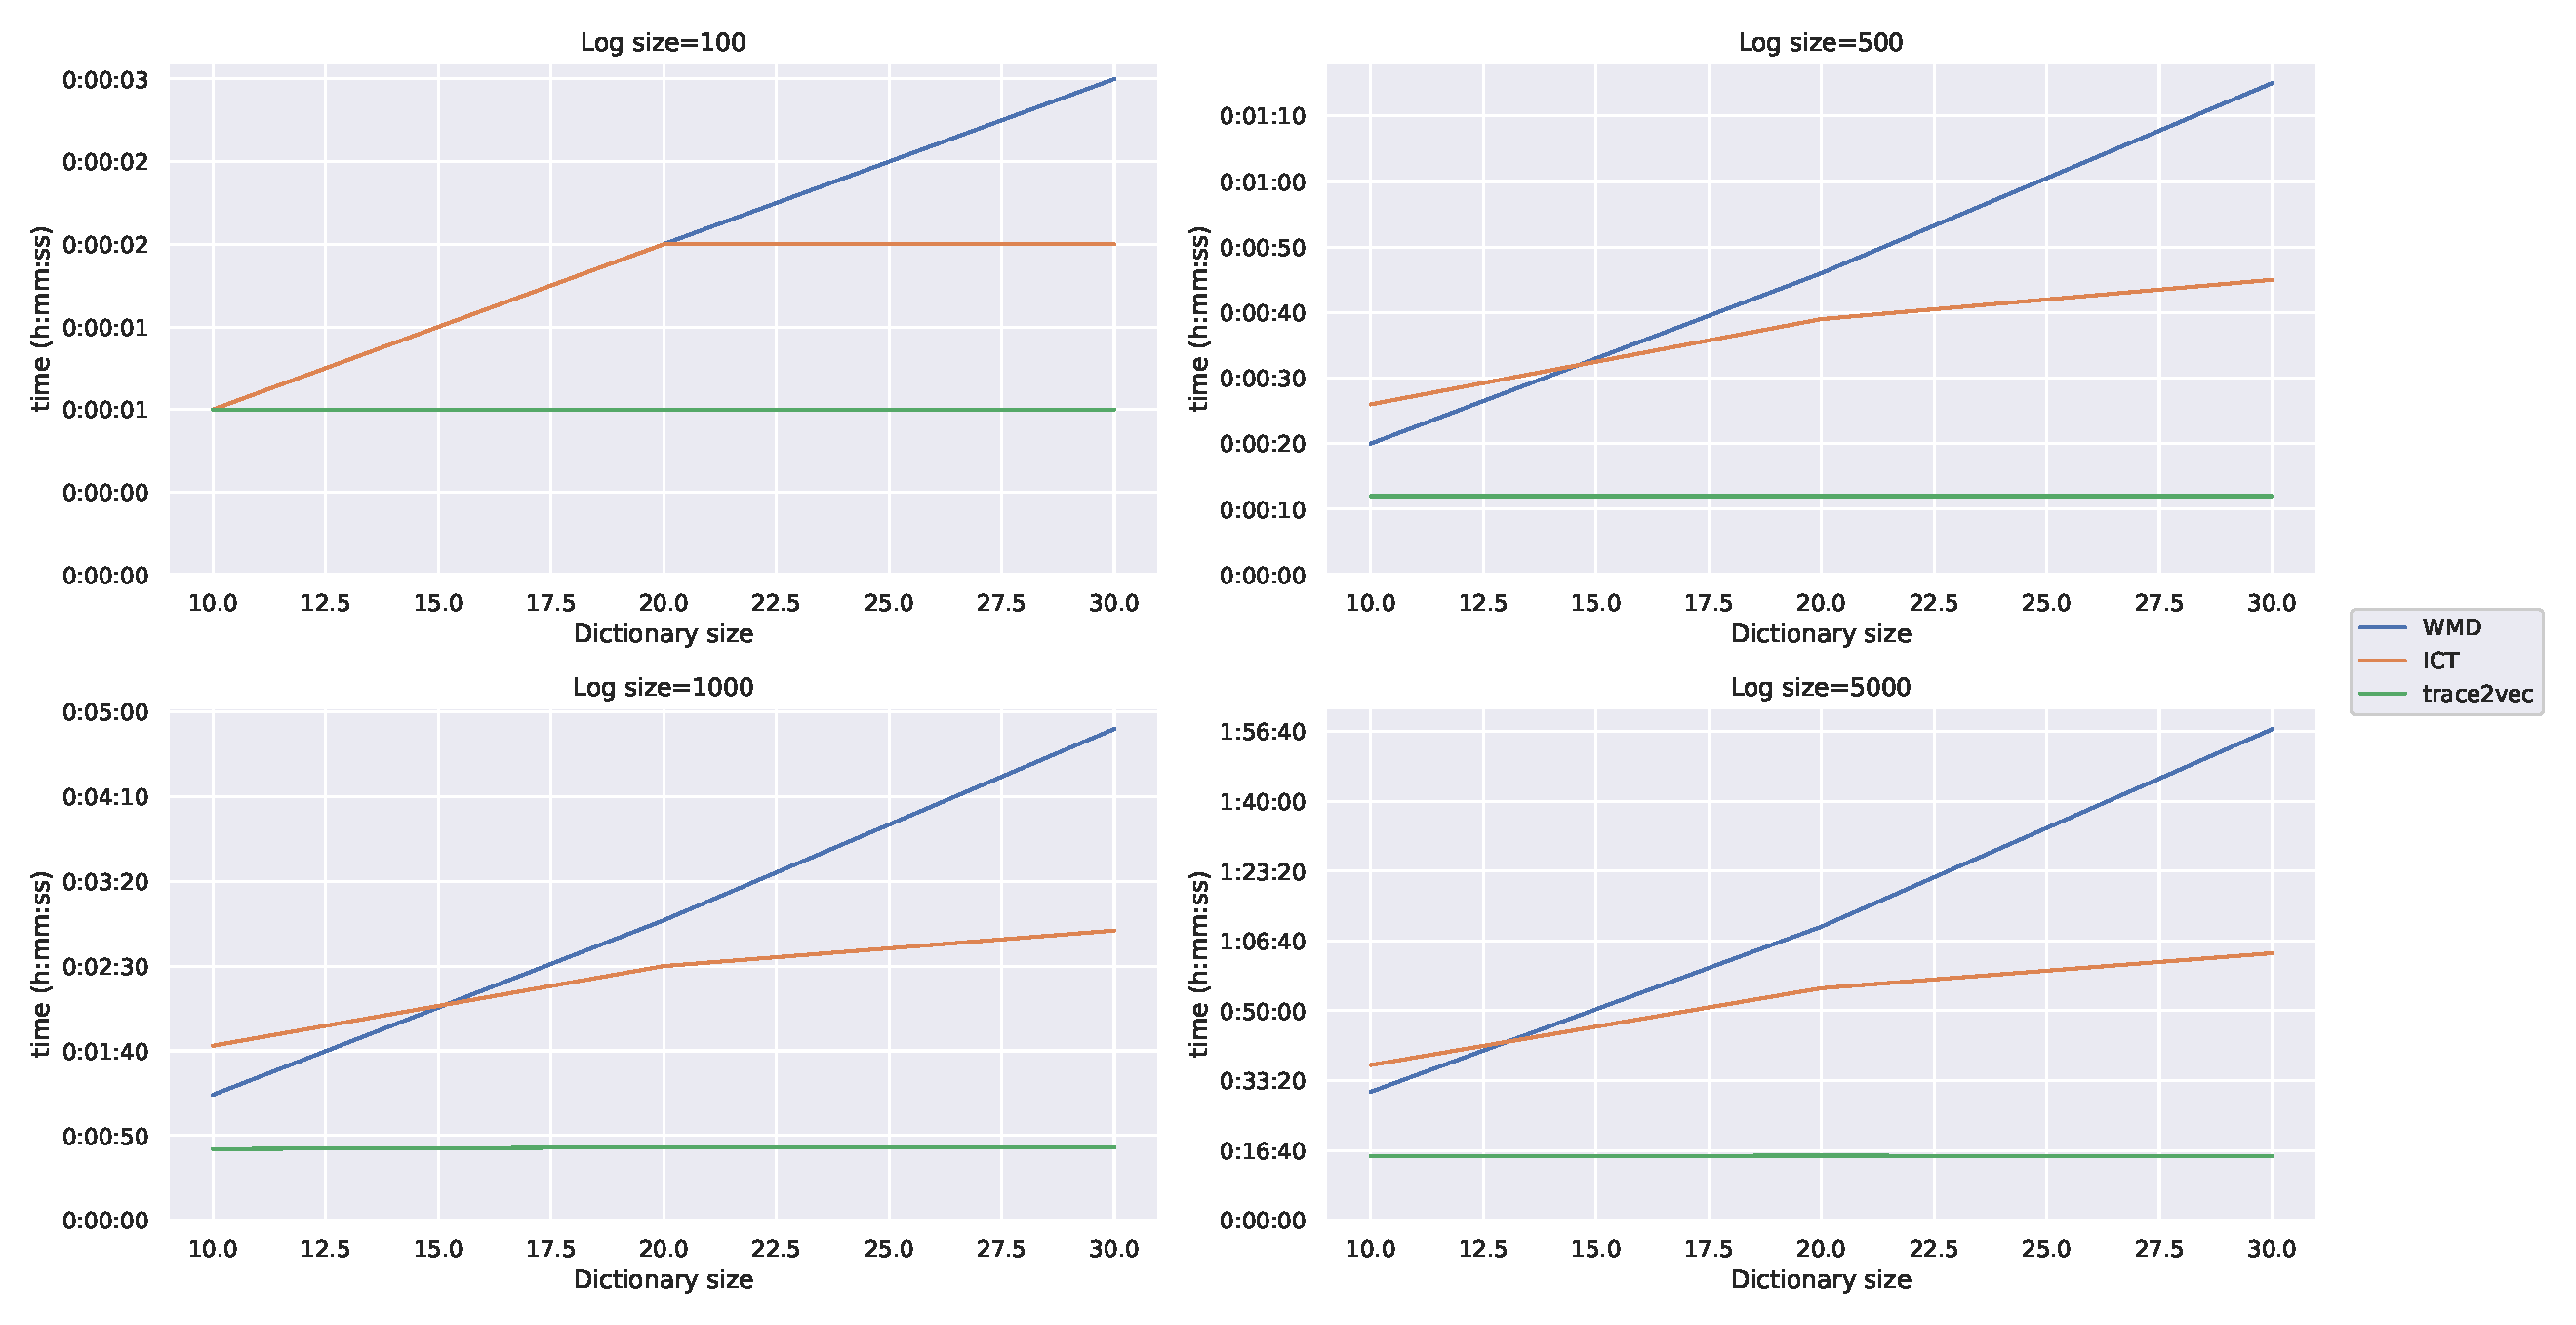
\includegraphics[width=1\textwidth]{figures/scaling}
			\caption{Runtimes for all three methods for varying sizes of logs and dictionaries.}
			\label{fig:scalability}
		\end{figure}
	\end{frame}
	
	
	\begin{frame}
		\frametitle{Scaling}
		\begin{itemize}
			\item unoptimized ICT already rivalling WMD, very likely attractive alternative.
			\item ICT scales well, \emph{trace2vec} stays the same with dictionary size
			\item All methods scale roughly quadratically with log-size, since the number of necessary comparisons grows quadratically
			\item log-comparison method. Performance dependent on model complexity. How many traces are needed to describe the model sufficiently well.
		\end{itemize}
	\end{frame}
	
	\section{Internet of Things}
	\begin{frame}
		\frametitle{Internet of Things}
		\begin{itemize}
			\item Better performance, and especially better scaling w.r.t. number of activities and trace length.
			\item Learned embeddings could be shared between devices, moving work out of the evaluation to a preceding training step.
			\item Embeddings have other advantages, no more binary activity equality, could allow for more fine grained conformance.
			\item Possibly much more complex tasks. E.g. an analogy to predictive text, i.e. predicting the next event given a sequence of observed events.
		\end{itemize}
	\end{frame}
	
\end{document}